\section{CFD model}
    Během výpočtů byl použit předpoklad stacionárního vazkého proudění ideálního plynu, od čehož se odvíjí i forma níže uvedených rovnic. 
    \subsection{Základní systém rovnic}
        
        \subsubsection{Rovnice kontinuity}
            Zákon zachování hmotnosti je pro stlačitelné stacionární proudění popsán následující rovnicí:
            \begin{equation} \label{eq:rovnice-kontinuity}
                \nabla \cdot  \brac{\rho \Vec{u}} = 0  
            \end{equation}
            \noindent kde $\rho \unit{\frac{kg}{m^3}}$ je hustota a $\Vec{u} \unit{\frac{m}{s}}$  je rychlost proudění.
        
        \subsubsection{Pohybová rovnice}
            Přenos hybnosti je popsán Navier-Stokesovými rovnicemi pro stacionární proudění:
            \begin{equation} \label{eq:pohybova-rovnice}
                \nabla \cdot \brac{\rho \Vec{u} \otimes \Vec{u}} = - \nabla p + \nabla \cdot \Tensor{\tau}
            \end{equation}
            \noindent kde $p \unit{Pa}$ je statický tlak a $\Tensor{\tau} \unit{\frac{N}{m^2}}$ je tenzor vazkých napětí daný následujícím vztahem:
            \begin{equation} \label{eq:tenzor-vazkych-napeti}
                \Tensor{\tau} = \mu \Brac{\nabla \Vec{u} + \nabla \Vec{u}^T - \frac{2}{3} \brac{\nabla \cdot \Vec{u}} \Tensor{I}}
            \end{equation}
            \noindent kde $\mu \unit{Pa s}$ je dynamická viskozita a $\Tensor{I} \unit{1}$ je jednotková matice.
            
        \subsubsection{Energetická rovnice}
            Řešení stlačitelného proudění vyžaduje doplnění energetické rovnice, kterou lze zapsat následovně:
            \begin{equation} \label{eq:energeticka-rovnice}
                \nabla \cdot \brac{\rho \Vec{u} H + \Vec{q} - \Tensor{\tau} \cdot \Vec{u}} = 0
            \end{equation}
            \noindent kde $H \unit{\frac{J}{kg}}$ je celková měrná entalpie a $\Vec{q} \unit{\frac{W}{m^2}}$ je vektor tepelného toku.
        \subsubsection{Konstitutivní vztahy}
        \smallSection{Stavová rovnice ideálního plynu}
        Rovnice popisuje vazbu mezi stavovými veličinami tekutiny:
        \begin{equation} \label{eq:stavova-rovnice}
            \frac{p}{\rho} = r T
        \end{equation}
        \noindent kde $T \unit{K}$ je termodynamická teplota a $r \unit{\frac{J}{kg K}}$ je měrná plynová konstanta, pro vzduch rovna $287.2 \Unit{\frac{J}{kg K}}$.
        
        \smallSection{Celková měrná entalpie}
        Měrnou entalpii proudění $h \unit{\frac{J}{kg}}$ lze určit ze vztahu:
        \begin{equation} \label{eq:entalpie}
            h = c_p T = e + \frac{p}{\rho} = c_v T + \frac{p}{\rho}
        \end{equation}
        \noindent kde $c_p \, , \; c_v  \unit{\frac{J}{kg K}}$ jsou měrné tepelné kapacity za konstantního tlaku, resp. konstantního objemu a $e \unit{\frac{J}{kg}}$ je měrná energie. Přičtením měrné kinetické energie proudění dostáváme celkovou měrnou entalpii $H$:
        \begin{equation} \label{eq:celkova-entalpie}
            H = h + \frac{\norm{\Vec{u}}^2}{2}
        \end{equation}

    \newpage
        
    \subsection{Model turbulence}

        Vzhledem k povaze řešených úloh byl zvolen dvourovnicový RANS (\textit{Reynolds Averaged Navier Stokes}) model turbulence $k-\omega$ SST (\textit{Shear Stress Transport}, viz Menter \cite{Menter1993,Menter1994}), který kombinuje výhody modelu $k-\varepsilon$ ve volném proudu a modelu $k-\omega$ ve vazké podvrstvě. Transportní rovnice pro $k-\omega$ SST mají následující tvar:
        \begin{equation} \label{eq:rovnice-pro-k} 
            \nabla \cdot \brac{\rho k \Vec{u}} = P_k - \beta ^* \rho \omega k + \nabla \cdot \Brac{\brac{\mu + \sigma _k \mu _t} \nabla k}
        \end{equation}
        \begin{equation} \label{eq:rovnice-pro-omega}
            \nabla \cdot \brac{\rho \omega \Vec{u}} = \frac{\gamma}{\nu _t} P_k - \beta \rho \omega ^2 + \nabla \cdot \Brac{\brac{\mu + \sigma _\omega \mu _t} \nabla \omega} + 2 \brac{1 - F_1} \frac{\rho \sigma _{\omega 2}}{\omega} \nabla k \cdot \nabla \omega
        \end{equation}
        \noindent kde $k \unit{\frac{m^2}{s^2}}$ je turbulentní kinetická energie, $\omega \unit{\frac{1}{s}}$ je specifická rychlost disipace, $\mu \unit{Pa s}$ je dynamická viskozita a $\beta, \beta^*, \gamma, \sigma _k, \sigma _\omega, \sigma _{\omega 2}$ jsou konstanty. $P_k$ představuje produkci turbulentní kinetické energie, která je s využitím limiteru dána vztahem:
        \begin{equation}
            P_k = \min \brac{\Tensor{\tau} : \nabla \Vec{u}, 20 \beta ^* \rho \omega k}
        \end{equation}
        kde $\Tensor{\tau}$ je tenzor turbulentního napětí určený vztahem:
        \begin{equation}
            \Tensor{\tau} = \mu _t \brac{\nabla \Vec{u} + \nabla \Vec{u} ^T - \frac{2}{3} \nabla \cdot \Vec{u} \Tensor{I}} - \frac{2}{3} \rho k \Tensor{I}
        \end{equation}
        Poslední člen rovnice \ref{eq:rovnice-pro-omega} představuje příčnou difuzi, zajišťující přechod mezi modely $k-\omega$ a $k-\varepsilon$. Ten je zprostředkovaný funkcí $F_1$:
        \begin{equation}
            F_1 = \tanh \Biggl\{ \min \Brac{ \max \brac{\frac{\sqrt{k}}{0.09 \omega y}, \frac{500 \nu}{y^2 \omega}, \frac{4 \rho \sigma _{\omega 2} k}{\var{CD}_{k \omega} y^2}}} \Biggr\} ^4  
        \end{equation}
        \noindent kde $y \unit{m}$ je vzdálenost od nejbližší stěny a $\var{CD}_{k \omega}$ odpovídá kladné části příčné difuze definované následujícím vztahem:
        \begin{equation}
            \var{CD}_{k \omega} = \max \brac{2 \rho \sigma _{\omega 2} \frac{1}{\omega} \nabla k \cdot \nabla \omega, 10^{-20}}
        \end{equation}
        Turbulentní vazkost $\nu _t$, respektive $\mu _t$, je definována jako:
        \begin{equation} \label{eq:turbulentni-vazkost}
            \nu _t = \frac{a_1 k}{\max \brac{a_1 \omega, \Omega F_2}} \hspace{1cm} \textrm{resp.} \hspace{1cm} \mu _t = \frac{\rho a_1 k}{\max \brac{a_1 \omega, \Omega F_2}}
        \end{equation}
        \noindent kde $\Omega$ představuje absolutní hodnotu vířivosti a $F_2$ je funkce daná vztahem:
        \begin{equation}
            F_2 = \tanh \Brac{\max \brac{2\frac{\sqrt{k}}{0.09 \omega y}, \frac{500 \nu}{y^2 \omega}}}^2
        \end{equation}
        \newpage
        Konstanty $\beta, \gamma, \sigma _k$ a $\sigma _\omega$ jsou s ohledem na polohu (stěna/volný proud) definovány pomocí funkce $F_1$:
        \begin{equation}
            \Phi = F_1 \Phi _1 + \brac{1 - F_1} \Phi _2
        \end{equation}
        \noindent kde $\Phi$ představuje libovolnou z konstant. Pro úplnou reprezentaci modelu je tak třeba definovat pro všechny konstanty jejich hodnotu pro model $k-\omega$ (index $1$) a pro model $k-\varepsilon$ (index $2$):

        \begin{table}[ht!]
            \centering
            \caption{Konstanty modelu k-$\omega$ SST \cite{Ansys2020Theory}.}
            \begin{tabular}{l|l|l|l|l|l|l|l|l}
                $\sigma _{k 1}$ & $\sigma _{\omega 1}$ & $\beta _1$ & $\sigma _{k 2}$ & $\sigma _{\omega 2}$ & $\beta _2$ & $\beta ^*$      & $\chi$               & $a_1$   \\ \hline
                $1.176$         & $2$                  & $0.075   $ & $1$             & $1.168$              & $0.0828$   & $0.09$          & $0.41$               & $0.31$  \\           
            \end{tabular}
            \label{tab:konstanty-turbulence}
        \end{table}

        \noindent Konstanty $\gamma _1$ a $\gamma _2$ jsou definovány následujícími vztahy:
        \begin{equation}
            \gamma _1 = \frac{\beta _1}{\beta ^*} - \frac{\sigma _{\omega 1} \chi ^2}{\sqrt{\beta ^*}}
        \end{equation}

        \begin{equation}
            \gamma _1 = \frac{\beta _2}{\beta ^*} - \frac{\sigma _{\omega 2} \chi ^2}{\sqrt{\beta ^*}}
        \end{equation}

    \newpage
    \subsection{Výpočetní geometrie}
        Vzhledem k charakteru řešeného problému byla geometrie proměnlivá. Jednotícím prvkem byla přítomnost alespoň jednoho ze dvou teplotních čidel, jehož restituční faktor byl zkoumán. Podle aktuální simulace se však měnilo uspořádání a přítomnost dalších geometrických prvků, jako například stínění.
    
        \subsubsection{Výpočetní oblast}
            Výpočty byly prováděny na geometrii umístěné v kontrolní oblasti tvaru válce o průměru $250 \Unit{mm}$ a délce $450 \Unit{mm}$. Vzhledem k rozměrům čidel, respektive celkové konstrukce, se jednalo o dostatečně velký kontrolní objem, jehož hranice neměly ovlivňovat proudění okolo sondy. Veškeré měřené geometrie byly ve válci umístěné $150 \Unit{mm}$ od vstupní oblasti, viz Obrázek \ref{fig:vypocetni-oblast}, ze kterého je patrné i umístění souřadného systému, na který bude dále v práci odkazováno.
            
            \begin{figure}[ht!]
                \centering
                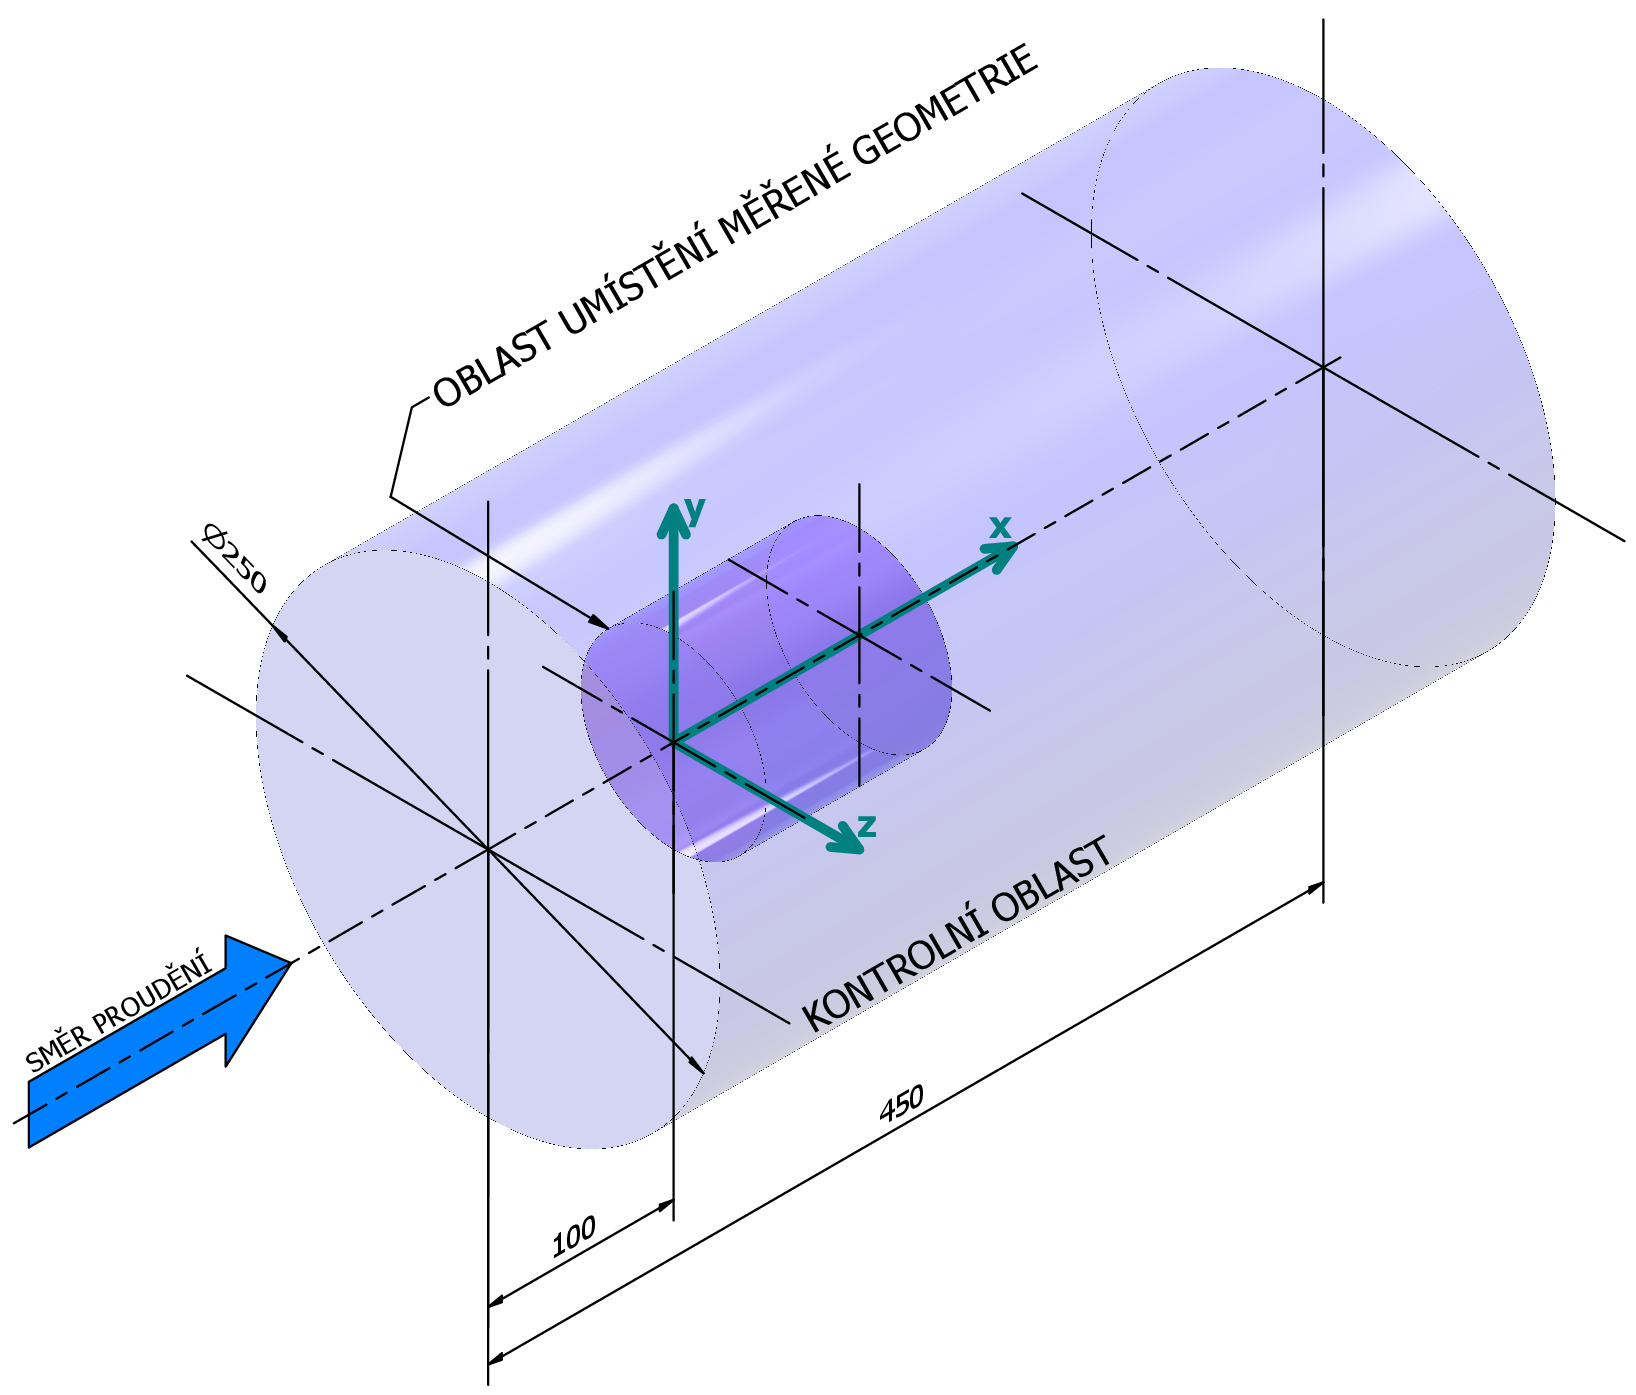
\includegraphics[width=\textwidth]{300_VYPOCETNI_MODEL/Vypocetni_oblast.png}
                \caption{Výpočetní oblast s vyznačením souřadného systému a polohy měřených geometrií.}
                \label{fig:vypocetni-oblast}
            \end{figure}
        
        \subsubsection{Využití symetrie}
            U všech zkoumaných geometrií se nacházela alespoň jedna rovina symetrie – bylo tedy možné využít této výhody pro úsporu výpočetního výkonu. Veškeré simulace uvedené v Kapitolách \ref{sec:konstrukcni-upravy} a \ref{sec:finalni-geometrie} s výjimkou analýzy směrové citlivosti v rovině $XZ$ byly provedeny s využitím symetrie výpočetního modelu, viz Obrázek \ref{fig:vypocetni-oblast-symetrie}.
            
            \begin{figure}[ht!]
                \centering
                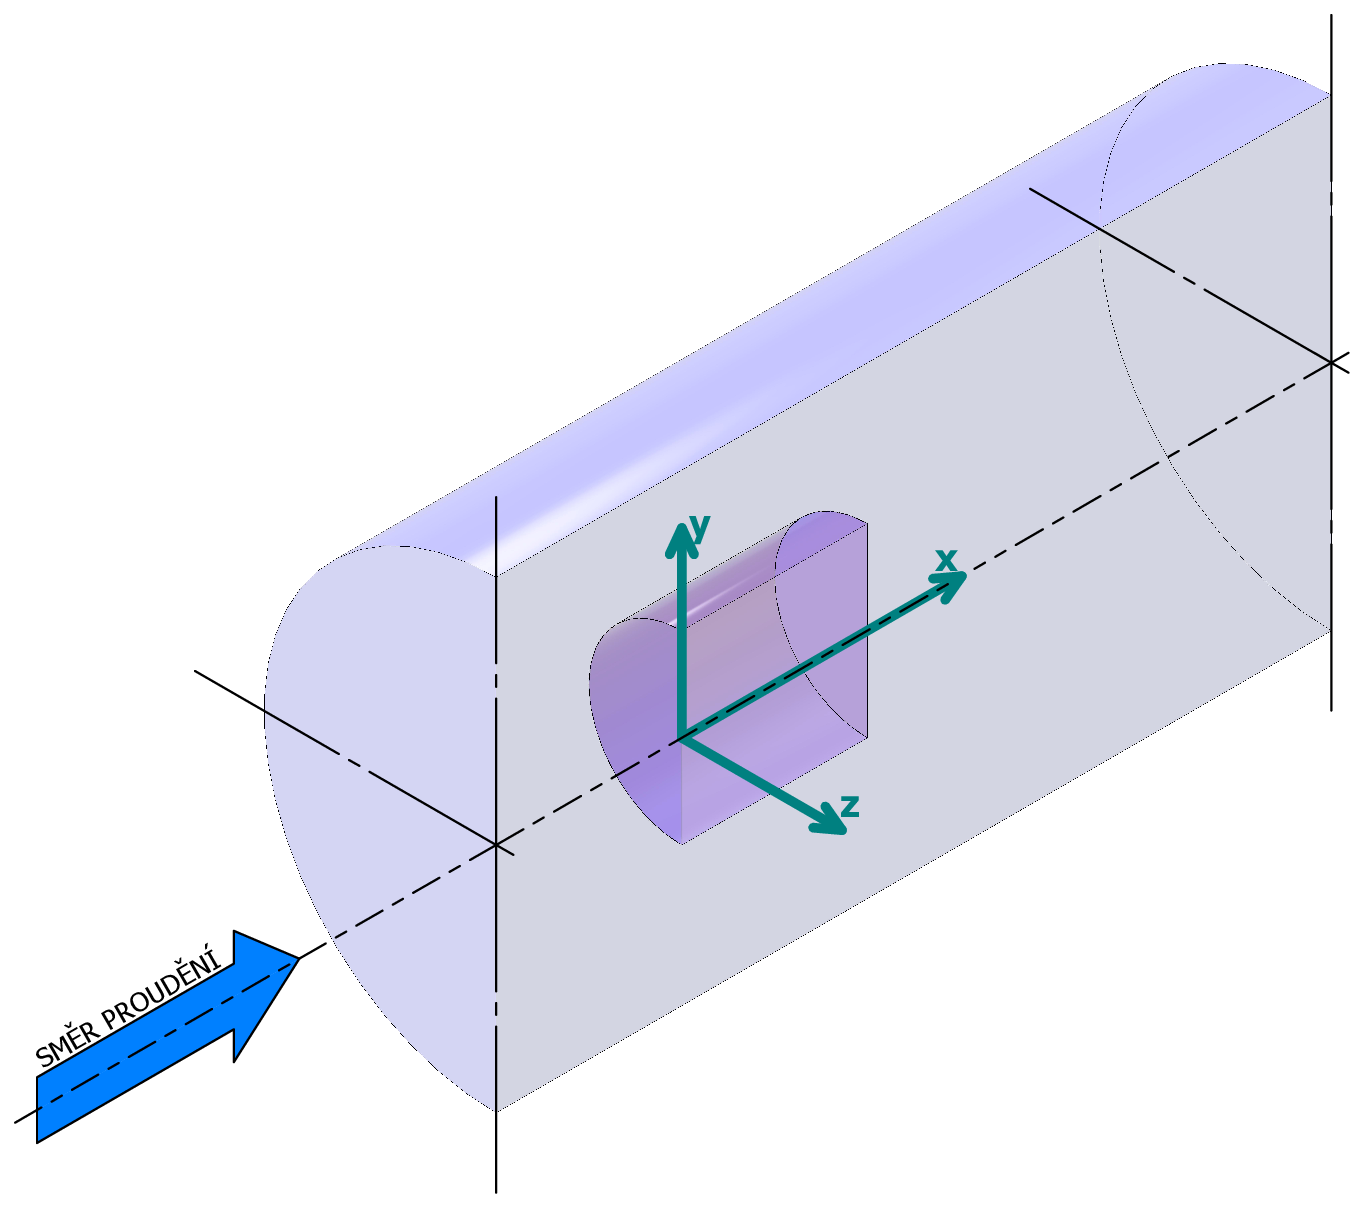
\includegraphics[width=\textwidth]{300_VYPOCETNI_MODEL/Vypocetni_oblast_symetrie.png}
                \caption{Výpočetní oblast pro řešení symetrických úloh.}
                \label{fig:vypocetni-oblast-symetrie}
            \end{figure}
         
	\newpage
        \subsubsection{Materiály} \label{sec:materialy}
            Během výpočtů byly uvažovány celkem tři materiály, ze kterých se skládala geometrie – trubice byla tvořena mosazí, čidla byla uvažována jako homogenní tělesa z keramiky $Al_2 O_3$ a těsnění bylo reprezentováno pryží. Použité fyzikální vlastnosti jednotlivých materiálů jsou uvedeny v Tabulce \ref{tab:materialy}.
            
            \renewcommand{\arraystretch}{2}
            \begin{table}[ht!]
                \centering
                \caption{Fyzikální vlastnosti použitých materiálů.}
                %\resizebox{.7\textwidth}{!}{%
                \begin{tabular}{l|l|l|l}
                                                                                  & Mosaz                        & Pryž                        &  Keramika                      \\ \hline
                    Hustota $\unit{\frac{kg}{m^3}}$                               & \multicolumn{1}{c|}{$8730$}  & \multicolumn{1}{c|}{$1100$} & \multicolumn{1}{c}{$3500$}     \\ \hline
                    Měrná tepelná kapacita $\unit{\frac{J}{kg K}}$          & \multicolumn{1}{c|}{$400$}   & \multicolumn{1}{c|}{$1300$} & \multicolumn{1}{c}{$700$}      \\ \hline
                    Tepelná vodivost $\unit{\frac{W}{m K}}$                 & \multicolumn{1}{c|}{$96$}    & \multicolumn{1}{c|}{$0.09$} & \multicolumn{1}{c}{$30$}      
                \end{tabular}%
                %}
                \label{tab:materialy}
            \end{table}
            
            Jako proudící médium byl uvažován vzduch splňující stavovou rovnici ideální plynu (viz Vztah \ref{eq:stavova-rovnice}) s následujícími vlastnostmi:

		\begin{table}[ht!]
			\centering
            \caption{Fyzikální vlastnosti vzduchu.}
			%\resizebox{.7\textwidth}{!}{%
			\begin{tabular}{l|l}
				Měrná plynová konstanta $\unit{\frac{J}{kg K}}$ & Poissonovo číslo $\unit{1}$ \\ \hline
				\multicolumn{1}{c|}{$287$}                                                                        & \multicolumn{1}{c}{$1.4$}                \\ \hline
				Tepelná vodivost $\unit{\frac{W}{m K}}$ & Dynamická viskozita $\unit{Pa \cdot s}$ \\ \hline				
				\multicolumn{1}{c|}{$2.42 \cdot 10^{-2}$}                          &  \multicolumn{1}{c}{$1.7894 \cdot 10^{-05}$}     
			\end{tabular}%
			%}
			\label{tab:vzduch}
		\end{table}
            
            
     \newpage      
    \subsection{Okrajové podmínky}
        \subsubsection{Hranice výpočetní oblasti}
			Hranice válcové kontrolní oblasti byla rozdělena na tři části s odlišnými okrajovými podmínkami – podstavy válce představovaly vstup a výstup a jeho plášť poté nenarušený proud (viz Obrázek \ref{fig:okrajove-podminky}). Ve všech oblastech byly předepsány hodnoty uvedené v Tabulce \ref{tab:spolecne-op}. Ve vstupní oblasti byla dále zadávána rychlost proudění, respektive velikost vektoru rychlosti a jeho směrové cosiny (využito při analýze směrové citlivosti). Hranice nenarušeného proudu měla předepisovánu hodnotu Machova čísla a směr proudění (opět ve formě směrových cosinů vektoru rychlosti). 

	     \begin{figure}[ht!]
                    \centering
                        \begin{subfigure}{0.3\textwidth}
                             \centering
                             \captionsetup{width=.9\linewidth}
                                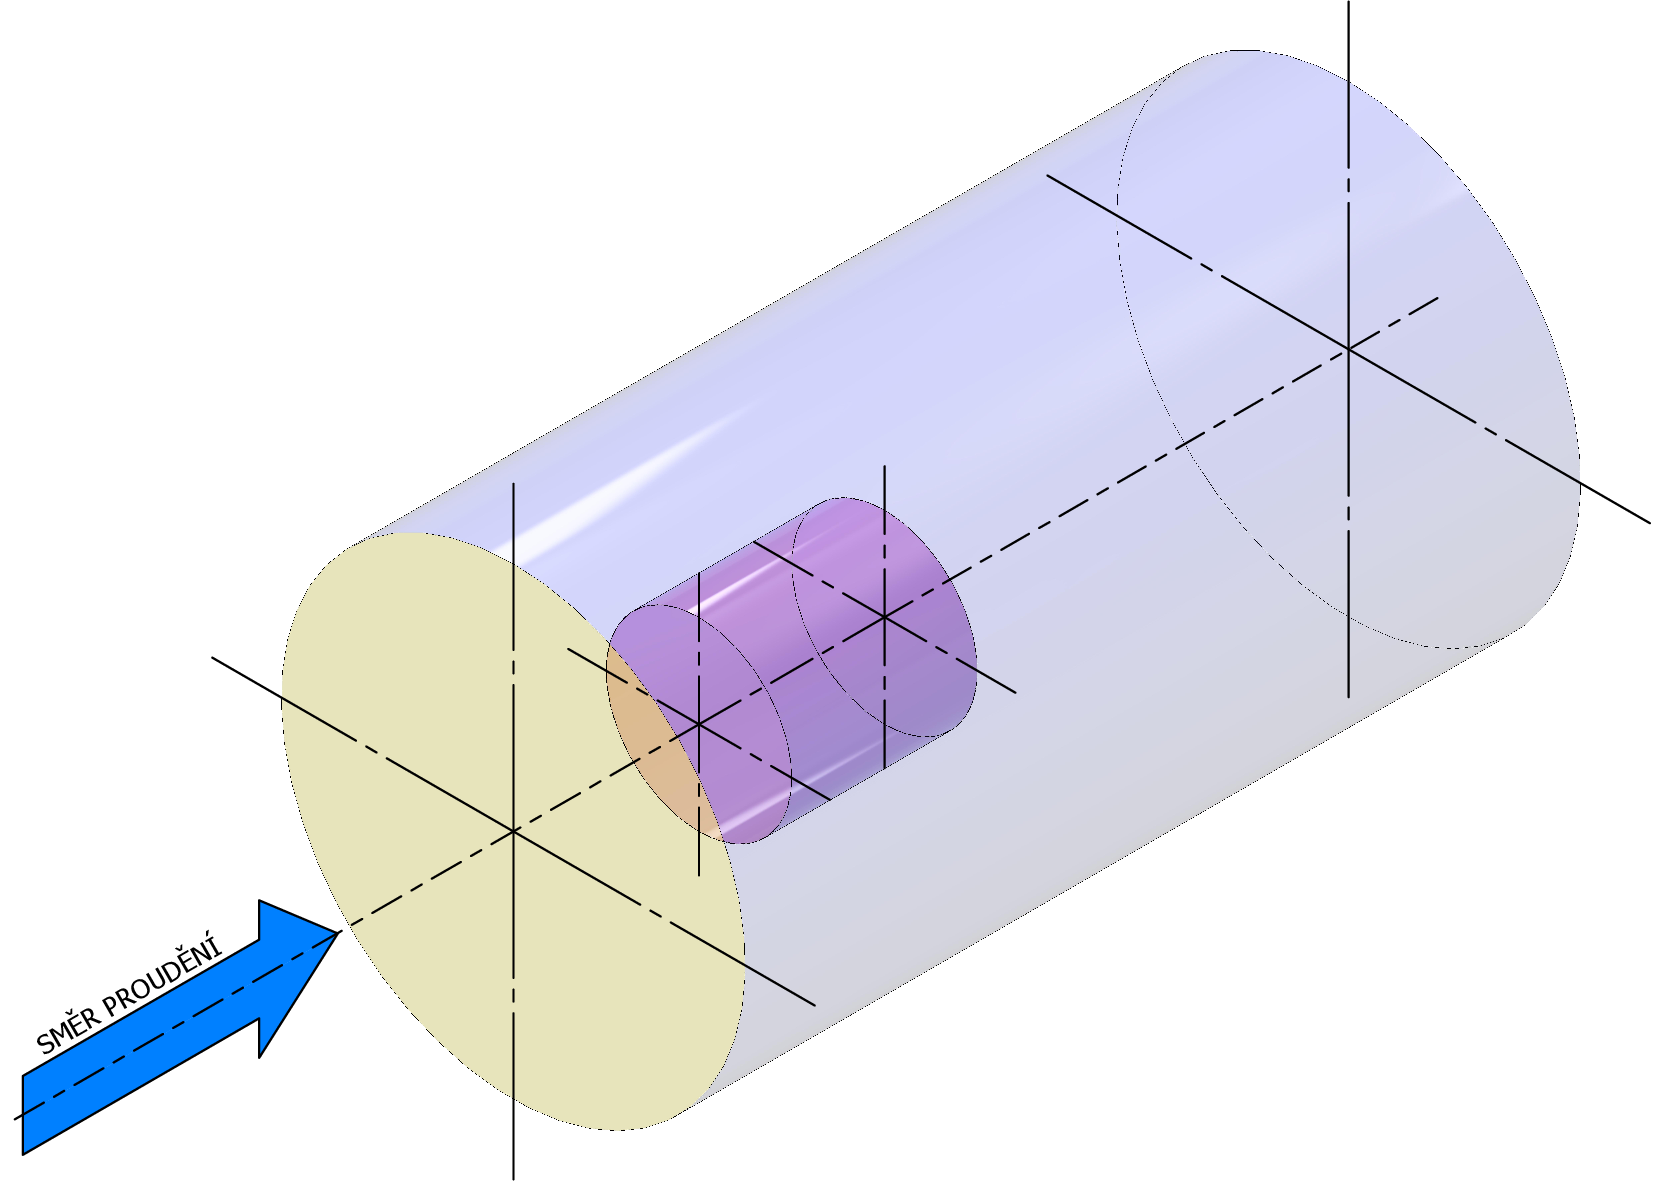
\includegraphics[width=\textwidth]{300_VYPOCETNI_MODEL/op-inlet.png}
                             \caption{Vstupní oblast.}
                             \label{fig:inlet}
                         \end{subfigure}
                         \begin{subfigure}{0.3\textwidth}
                             \centering
                             \captionsetup{width=.9\linewidth}
                             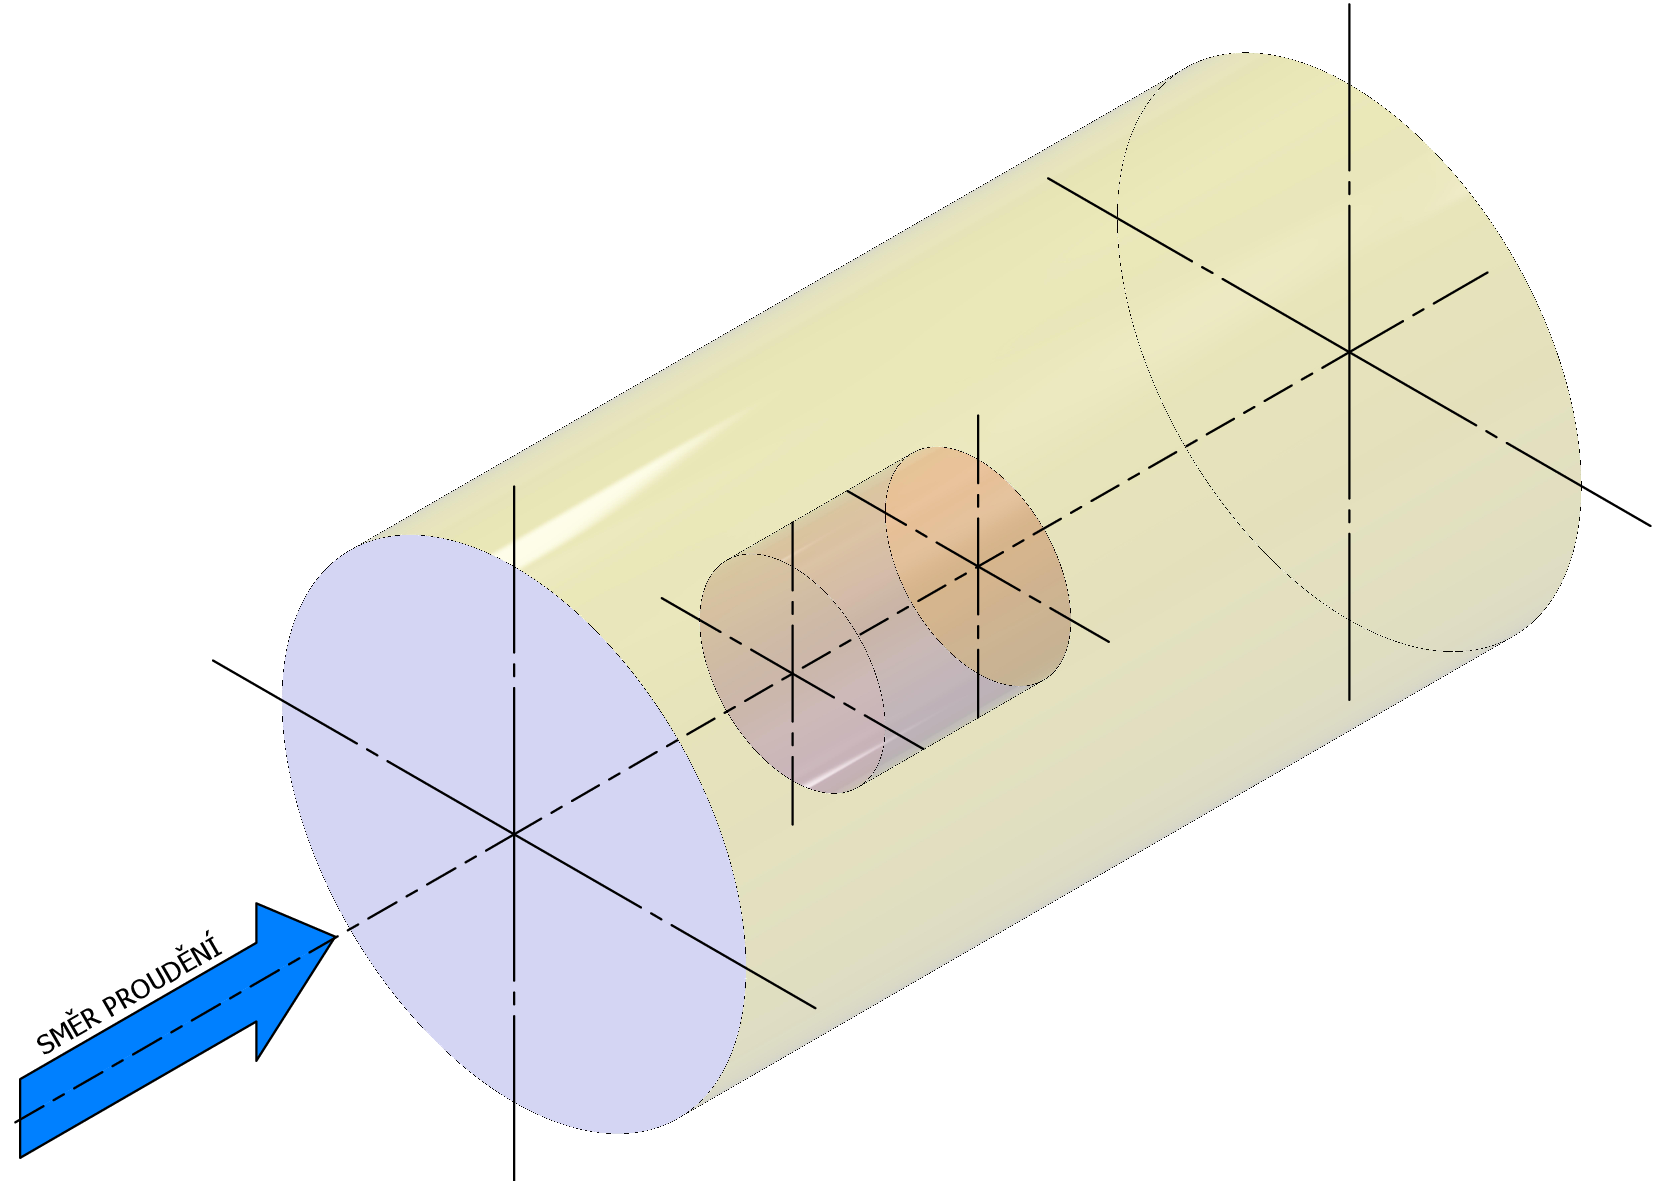
\includegraphics[width=\textwidth]{300_VYPOCETNI_MODEL/op-farfield.png}
                             \caption{Nenarušený proud.}
                             \label{fig:farfield}
                         \end{subfigure}
					\begin{subfigure}{0.3\textwidth}
                             \centering
                             \captionsetup{width=.9\linewidth}
                             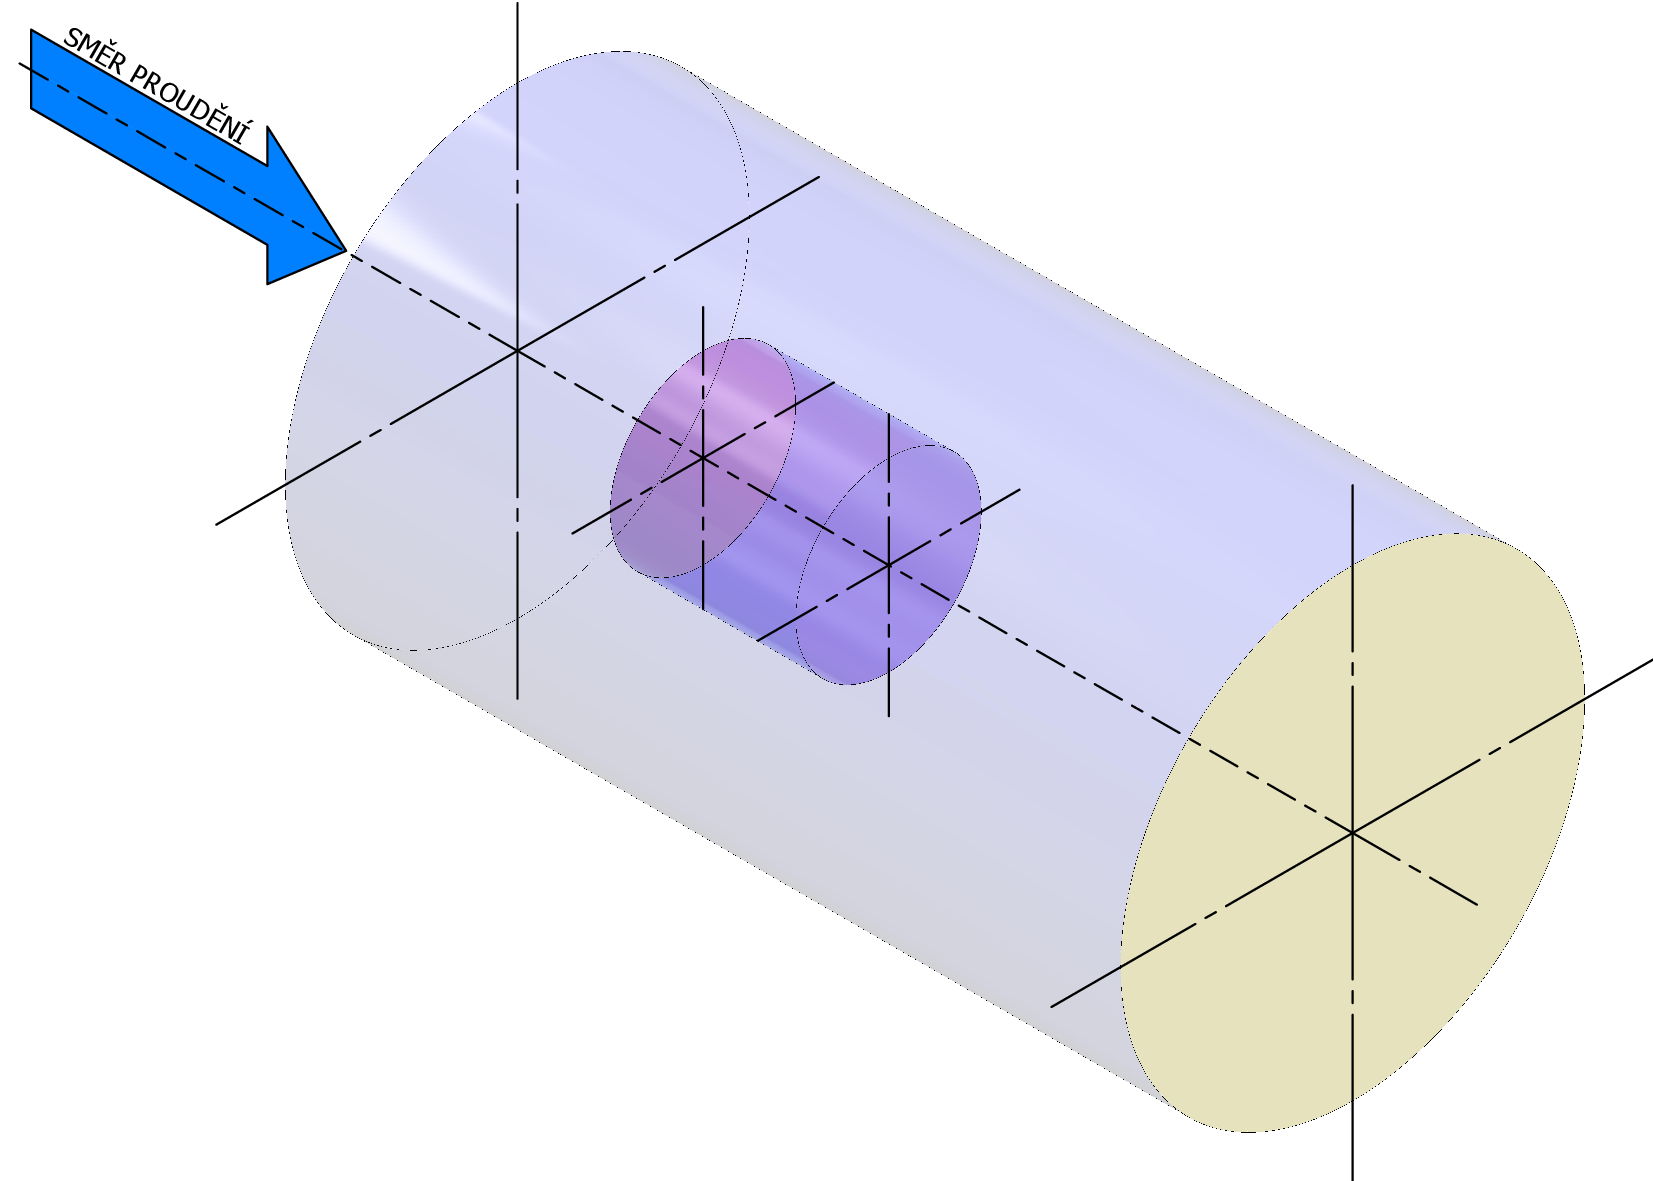
\includegraphics[width=\textwidth]{300_VYPOCETNI_MODEL/op-outlet.png}
                             \caption{Výstupní oblast.}
                             \label{fig:outlet}
                         \end{subfigure}
                    \caption{Části hranice pro aplikování okrajových podmínek (v jednotlivých obrázcích označeny žlutou barvou).}
                    \label{fig:okrajove-podminky}
         \end{figure}

         \begin{table}[ht!]
            \centering
            \caption{Hodnoty předepisované na hranici kontrolní oblasti.}
            %\resizebox{.7\textwidth}{!}$ & Směšovací délka $\unit{m}$  \\ \hline
                \multicolumn{1}{c|}{2.5}         & \multicolumn{1}{c}{0.01}   
            \end{tabular}%
            %}
            \label{tab:spolecne-op}
        \end{table}

         Výchozí rychlostí použitou pro testování bylo $250 \Unit{\frac{m}{s}}$, tomu odpovídá při teplotě $300 \Unit{K}$ Machovo číslo $0.72$. Nebude-li dále uvedeno jinak, pak byly pro výpočet použity právě tyto hodnoty.
			
        
        \subsubsection{Stěny}
            Při numerických simulacích bylo pro vyhodnocení restitučních faktorů třeba počítat s přestupem tepla do pevných látek a s jeho šířením objemem. V místech kontaktu proudícího média se stěnami geometrie byla proto použita podmínka sdílené teploty – teplota na hranici tekutiny byla přenesena na hranici tělesa.

    \newpage
    \subsection{Výpočetní síť} \label{sec:vypocetni-sit}
        Vytváření modelů probíhalo v prostředí software Autodesk Inventor (verze 2021 a 2022), odkud byly následně vyexportovány ve formátu \textit{.dwg}. K přípravě pro síťování byl následně použit software Ansys SpaceClaim (verze 2020b-2021b), jehož účel spočíval primárně ve sdílení topologie modelu, vytváření jmenných sekcí a exportu do optimalizovaného formátu \textit{.pmdb}. Samotné síťování poté probíhalo v software Ansys Fluent (verze 2020b-2021b).
        \subsubsection{Povrchová síť}
            Prvním krokem při vytváření výpočetní sítě pro řešič bylo importování geometrie (soubor \textit{.pmdb}) a vysíťování jejích ploch pomocí triangulace. Zde bylo použito následující nastavení:

            \begin{table}[ht!]
                \centering
                \caption{Předepisované hodnoty při vytváření povrchové sítě.}
                \begin{tabular}{l|l}
                    $\frac{\textrm{Minimální}}{\textrm{Maximální}}$ velikost elementů $\unit{mm}$                                            & Poměrný růst velikosti elementů $\unit{1}$ \\ \hline
                    \multicolumn{1}{c|}{$\frac{0.1}{15}$}                                                              & \multicolumn{1}{c}{$1.2$}                  \\ \hline
                    Maximální úhel překlenutí $\unit{deg}$                                                         & Minimální dělení hran $\unit{1}$           \\ \hline
                    \multicolumn{1}{c|}{$10$}                                                                      & \multicolumn{1}{c}{$3$}                     
                \end{tabular}
                \label{tab:povrchova-sit-nastaveni}
            \end{table}

            Kvalita povrchové sítě byla následně kontrolována, aby šikmost žádného elementu nepřesáhla $0.5$. Šikmost představuje odchylku geometrie buňky od optimálního tvaru (v případě triangulace se jedná o rovnostranný trojúhelník). Její hodnota se pohybuje mezi $0 \div 1$, kde $0$ odpovídá nejlepší kvalitě. Pro správný průběh a konvergenci výpočtů je doporučeno, aby maximální šikmost nepřesahovala $0.95$ a aby se průměrná šikmost pohybovala nejvýše okolo hodnoty $0.33$ \cite{Ansys2020User}. Tato doporučení platí pro konečnou objemovou síť, která se používá během výpočtů, nicméně počáteční kvalita povrchové sítě má zásadní vliv na jakost následujícího síťování.
        \subsubsection{Zjemnění v mezní vrstvě}
            Pro dosažení přijatelné přesnosti výpočtu přestupu tepla ze vzduchu do těles bylo třeba, s ohledem na použitý model turbulence, vytvořit dostatečně jemnou síť v oblasti mezní vrstvy tak, aby se bezrozměrná vzdálenost od stěny $y _+$ ($y _+ = \frac{u _\tau y}{\nu}$, kde $u _\tau \unit{\frac{m}{s}}$ je třecí rychlost) pohybovala v oblasti vazké podvrstvy. K tomu byly využity prismatické buňky v místech kontaktu tekutiny s měřenou geometrií. Cílem bylo dosažení průměrné $y_+$ co nejblíže jedné. Toho bylo docíleno pomocí nastavení uvedeného v Tabulce \ref{tab:mezni-vrstva-nastaveni}. Příklad rozložení $y_+$ podél povrchu teplotního čidla je uveden na Obrázku \ref{fig:yplus-stineni-A}.

            \begin{table}[ht!]
                \centering
                \begin{tabular}{ll}
                    \multicolumn{2}{l}{Míra natažení prvního elementu (\textit{aspect ratio}) $\unit{1}$}                            \\ \hline
                    \multicolumn{2}{c}{$6.2$}                                                                        \\ \hline
                    \multicolumn{1}{l|}{Poměrný růst velikosti elementů $\unit{1}$} & Počet prismatických vrstev $\unit{1}$ \\ \hline
                    \multicolumn{1}{c|}{$1.2$}                                      & \multicolumn{1}{c}{$10$}                
                \end{tabular}
                \caption{Předepisované hodnoty při vytváření prismatických buněk.}
                \label{tab:mezni-vrstva-nastaveni}
            \end{table}

            \begin{figure}[ht!]
                \centering
                \includegraphics*[width=\textwidth  ]{300_VYPOCETNI_MODEL/yplus-stineni-A.eps}
                \caption{Graf četností hodnot bezrozměrné vzdálenosti od stěny čidla A pro úlohu z Kapitoly \ref{sec:stineni-A}. Průměrná hodnota byla pro tento případ rovna $0.945$.}
                \label{fig:yplus-stineni-A}
            \end{figure}

            \newpage


        \subsubsection{Objemová síť}

        Při vytváření objemové sítě byly zvoleny polyhedrální buňky, které umožňují dosahovat přesnějších řešení oproti starším typům elementů při shodných počtech buňek. Umožňují navíc lepší odhad gradientu díky vyššímu počtu stěn a obecně lze s jejich použitím dosahovat lepší kvality sítě \cite{Sosnowski2018}. Postup generování objemové sítě byl následující:

        \begin{enumerate}
            \item Konverze povrchové triangulace na polygonální síť
            \item Vygenerování vrstev prismatických buněk
            \item Iterační generování polyhedrální objemové sítě ve zbytku objemu
        \end{enumerate}

        Maximální šikmost hotové sítě se vždy pohybovala pod hodnotou $0.85$. Počty buňek se pohybovaly v rozmezí $450 \div 550$ tisíc pro symetrické úlohy a $850 \div 950$ tisíc pro úlohy bez využití symetrie. Příklad výpočetní sítě je uveden na obrázku \ref{fig:sit-detail-stineni-A}.

        \begin{figure}
            \centering
            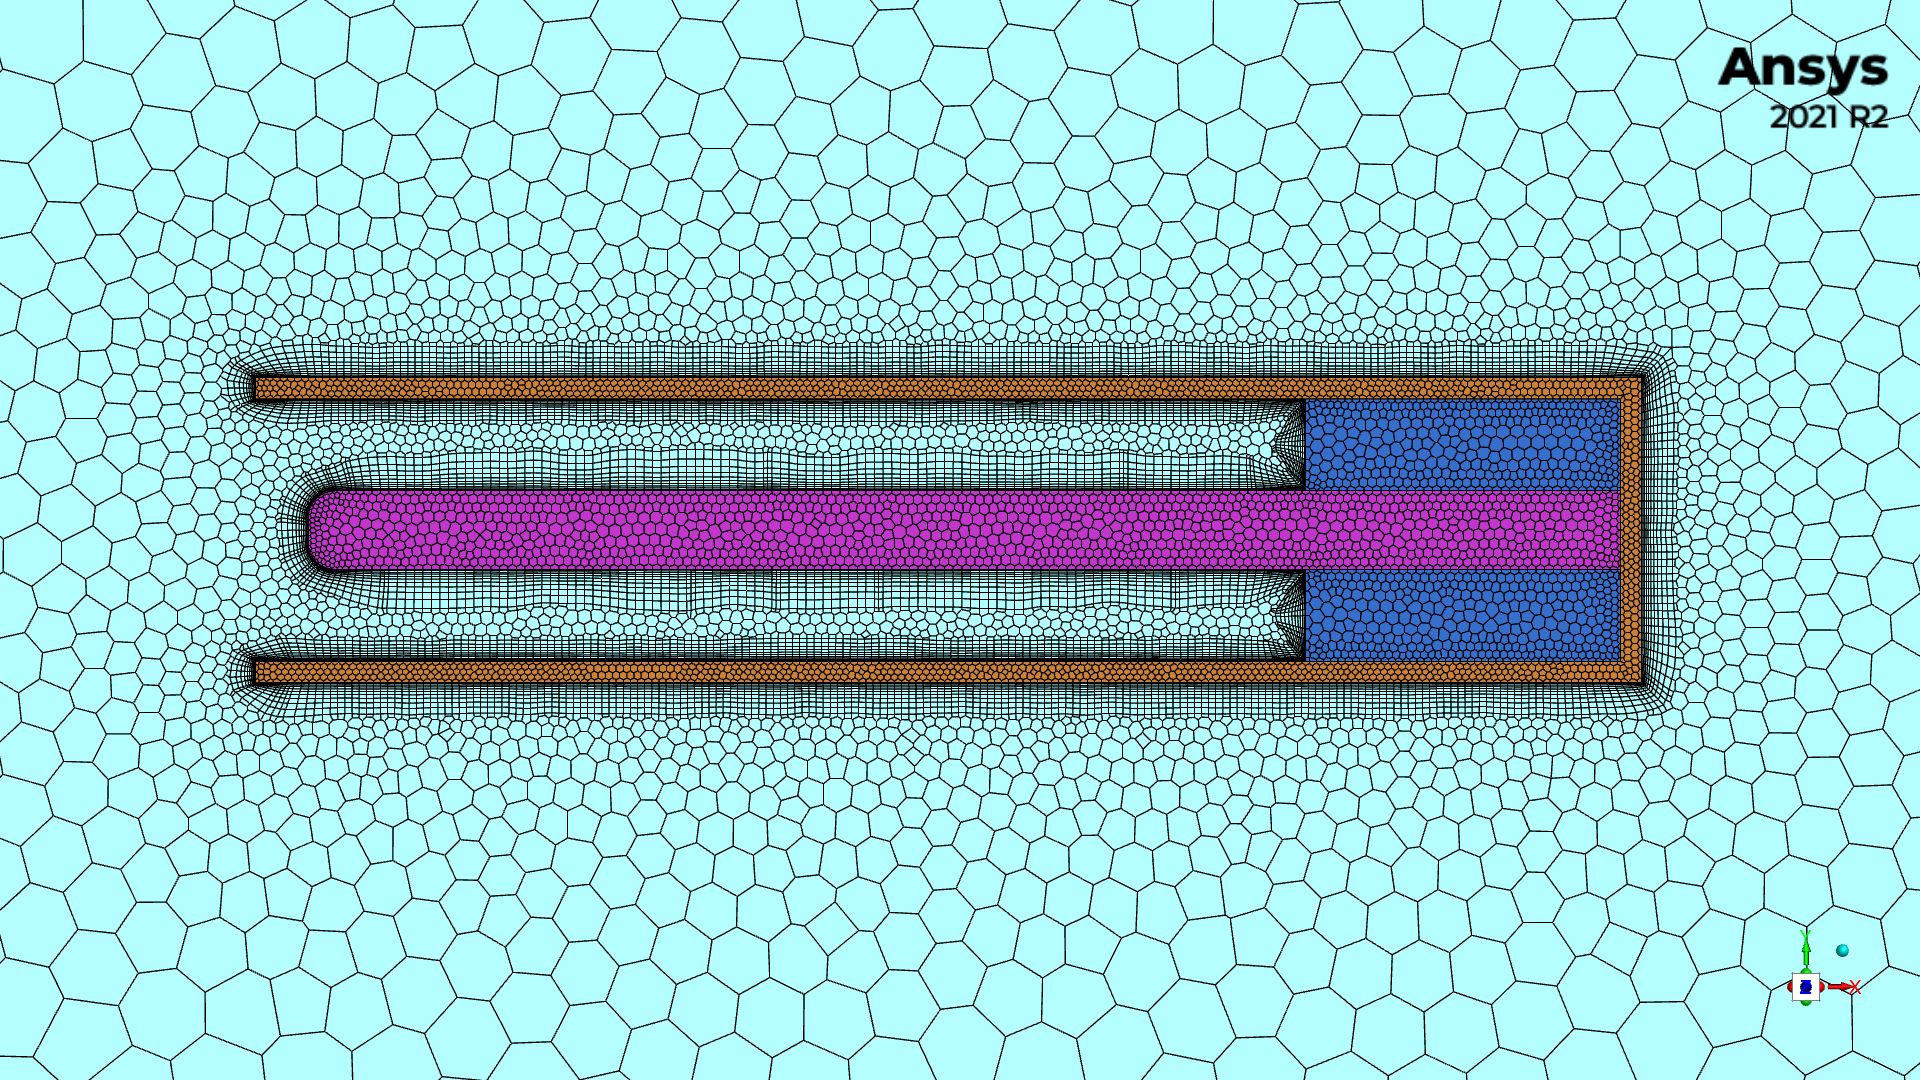
\includegraphics[width=\textwidth]{300_VYPOCETNI_MODEL/mesh_sym_odvetrani_A.png}
            \caption{Pohled na výpočetní síť z Kapitoly \ref{sec:stineni-A} ze strany symetrie.}
            \label{fig:sit-detail-stineni-A}
        \end{figure}
        
    \subsection{Numerický řešič}
        Veškeré výpočty byly provedeny v prostředí výpočetního software Ansys Fluent (verze 2020b-2021b). Ten využívá k řešení problémů metodu konečných objemů, která je pro úlohy počítačové dynamiky tekutin typická. Metoda spočívá v rozdělení kontrolní oblasti na vzájemně disjunktní kontrolní objemy, které ji kompletně pokrývají. Řešené rovnice jsou následně integrovány právě přes dané objemy a poté prostřednictvím diskretizace převedeny na soustavu lineárních rovnic. Způsoby diskretizace a odhadů popsané níže vycházejí z programové dokumentace pro Ansys Fluent 2020 \cite{Ansys2020Theory}.
        \subsubsection{Odhad gradientu} \label{sec:odhad-gradientu}
            Pro určení gradientu ve středu buněk byla zvolena, s ohledem na použití polyhedrální sítě, metoda nejmenších čtverců. Ta spočívá v hledání váhové funkce mezi dílčími gradienty $\brac{\nabla \varphi}_{c0,i}$:
            \begin{equation}
                \brac{\nabla \varphi}_{c0,i} \cdot \Vec{r_i} = \varphi _{ci} - \varphi _{c0} = \brac{\Delta \varphi} _i
            \end{equation}
            \noindent kde $\Vec{r_i}$ je vektor spojující středy buněk $c_0$ a $c_i$ a $\varphi _{c0}$, respektive $\varphi _{ci}$, jsou jim odpovídající hodnoty libovolné veličiny (viz Obrázek \ref{fig:urceni-gradientu}). 
            \begin{figure}[ht!]
                \centering
                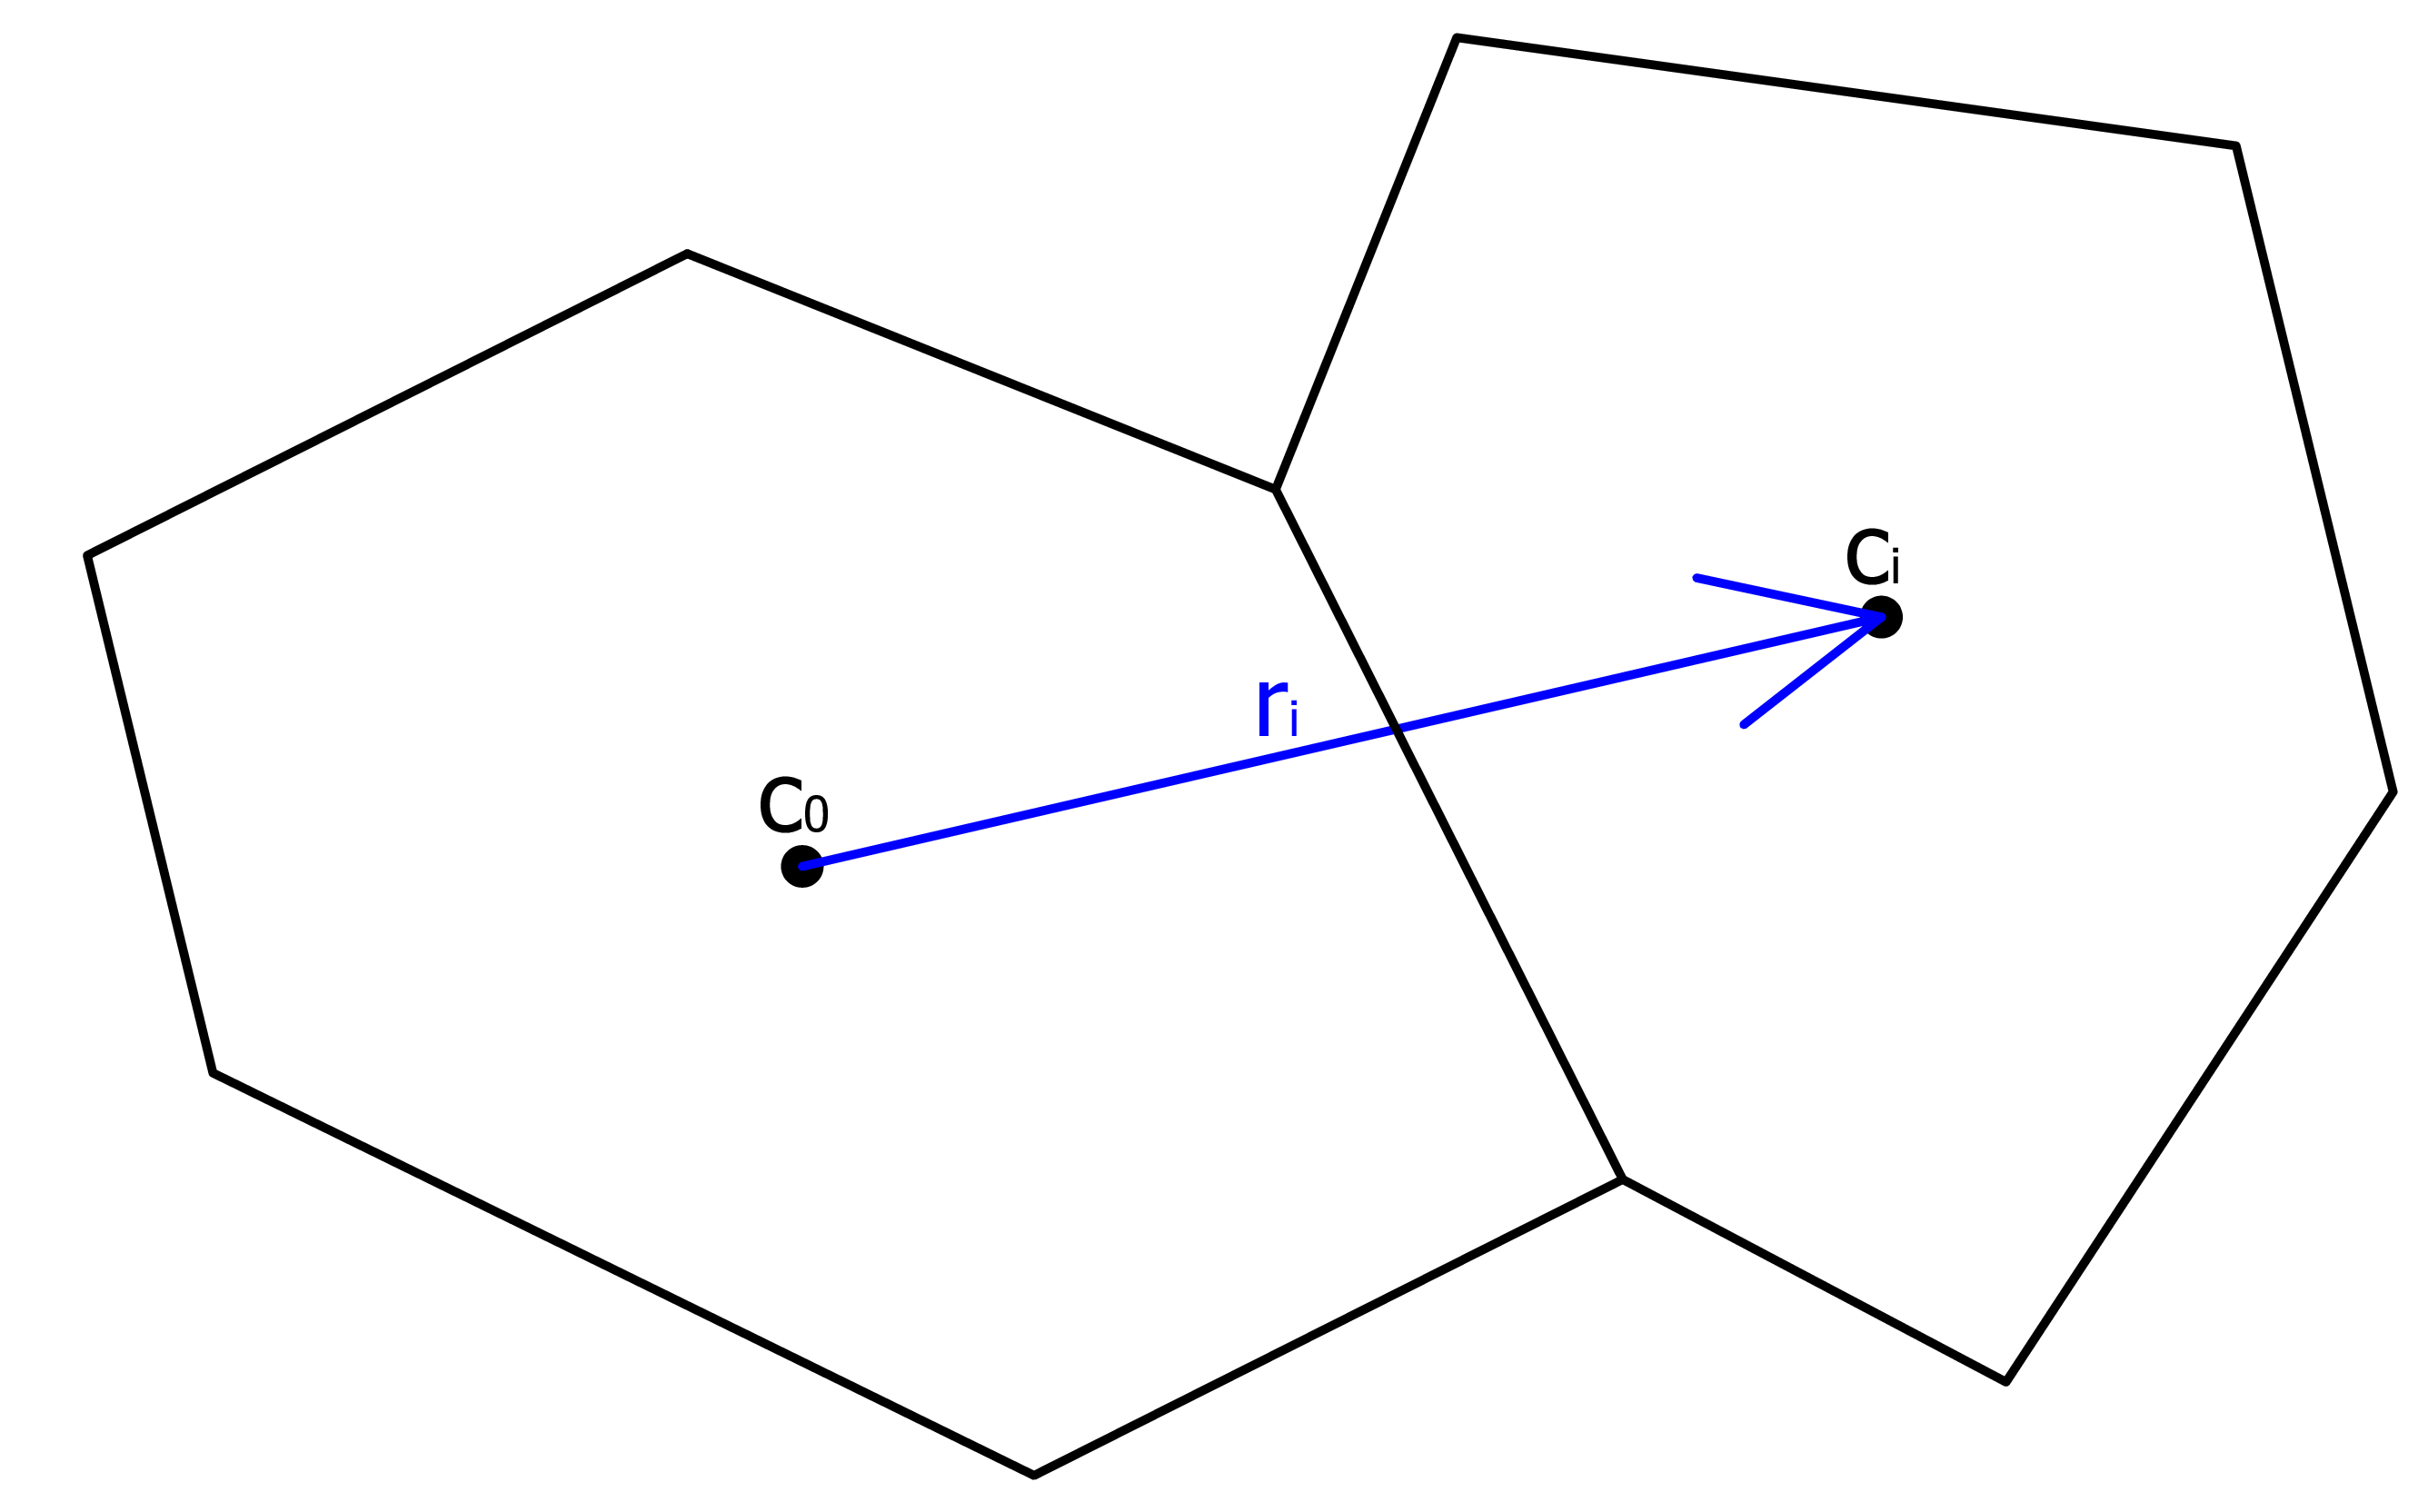
\includegraphics[width=.75\textwidth]{300_VYPOCETNI_MODEL/urceni_gradientu.png}
                \caption{Schéma pro určení gradientu pomocí metody nejmenších čtverců.}
                \label{fig:urceni-gradientu}
            \end{figure}
            Počet takto vzniklých gradientů je roven počtu sousedních buněk $n$, je tak třeba najít váhovou funkci $\Tensor{W}$, jejíž aplikací na soustavu rozdílů $\Vec{\Delta \varphi}$ získáme konečný gradient $\brac{\nabla \varphi} _{c0}$, tedy:
            \begin{equation}
                \brac{\nabla \varphi} _{c0} = \begin{pmatrix}
                    \brac{\nabla \varphi} _{c0} ^x \\
                    \brac{\nabla \varphi} _{c0} ^y \\
                    \brac{\nabla \varphi} _{c0} ^z 
                \end{pmatrix} = \begin{pmatrix}
                    W_{x1} & W_{x2} & \cdots & W_{xn} \\
                    W_{y1} & W_{y2} & \cdots & W_{yn} \\
                    W_{z1} & W_{z2} & \cdots & W_{zn} 
                \end{pmatrix} \begin{pmatrix}
                    \brac{\Delta \varphi} _1 \\
                    \brac{\Delta \varphi} _2 \\
                    \vdots \\
                    \brac{\Delta \varphi} _n
                \end{pmatrix} = \Tensor{W} \Vec{\Delta \varphi}
            \end{equation}
        \subsubsection{Aproximace hodnot na stěnách}
            Ansys Fluent využívá při výpočtech tzv. cell-centered formulaci metody konečných objemů – všechny veličiny jsou definovány ve středech buněk. Pro výpočet toků konečnými objemy je ale nutné znát také hodnoty veličin na jejich stěnách. K tomu byla zvolena metoda upwind druhého řádu přesnosti (\textit{linear upwind}). Její princip je založen na určení buňky \uv{proti proudu} $c _U$, obvykle s využitím vnější normály stěny, a následné extrapolaci hodnot z jejího středu do středu příslušné stěny:
            \begin{equation}
                \varphi _{f} = \varphi _U + \brac{\nabla \varphi} _U \cdot \Vec{r _f}
            \end{equation}
            \noindent kde $\varphi _f$ je hodnota libovolné veličiny ve středu stěny, $\varphi _U$ je hodnota ve středu buňky proti proudu, $\brac{\nabla \varphi} _U$ je gradient buňky proti proudu (viz Kapitola \ref{sec:odhad-gradientu}) a $\Vec{r_f}$ je vektor spojující střed buňky proti proudu a střed stěny.

            Určení tlaku na stěnách buněk se liší od všech ostatních veličin. V tomto případě byla namísto metody upwind použita centrální náhrada druhého řádu přesnosti:
            \begin{equation}
                p _{f} = \frac{p_{ci} + p _{c0}}{2} + \frac{\brac{\nabla p} _{ci} + \brac{\nabla p} _{c0}}{2}
            \end{equation}
        \subsubsection{Numerické schéma}
            Pro řešení bilančních rovnic bylo zvoleno sdružené schéma – narozdíl od sekvenčních algoritmů (například SIMPLE, PISO, \dots), které řeší postupně rovnice pro rychlost a následně pro tlak, sdružený algoritmus sestavuje soustavu rovnic řešící zároveň rychlostní i tlakové pole. Ta je poté řešena buď pomocí Gauss-Seidelovy iterační metody nebo pomocí metod založených na LU dekompozici \cite{Ansys2020Theory}.

            Výhoda sdruženého algoritmu spočívá u stacionárních úloh zejména v rychlosti konvergence \cite{Ansys2020User} – při testování vhodného schématu pro výpočty prezentované v této práci bylo s využitím sdruženého schématu dosaženo konvergence po přibližně $10\times$ méně iteracích, než tomu bylo u schématu SIMPLE.
        \subsubsection{Inicializace výpočtu}
            Iterační proces řešení vyžaduje počáteční vyplnění hodnot v kontrolních objemech. K tomu lze přistoupit několika způsoby, zde byla zvolena takzvaná hybridní inicializace. Ta spočívá v řešení Laplaceovy rovnice pro rychlostní potenciál $\varphi$ a pro tlak $p$ (viz Rovnice \ref{eq:incializace}) se zjednodušenými okrajovými podmínkami. Ostatní veličiny (teplota, turbulentní parametry, \dots) jsou v celém objemu voleny jako konstantní. 
            \begin{equation} \label{eq:incializace}
                \begin{split}
                    \Delta \varphi = 0 \\
                    \Delta p = 0
                \end{split}
            \end{equation}
            Využití hybridní inicializace, podobně jako použití sdruženého algoritmu, vedlo během výpočtů k jejich rychlejší konvergenci a bylo tak preferováno.
        \subsubsection{Určení restitučních faktorů}
            Vnitřní geometrie teplotních čidel byla během výpočtů idealizována (uvažovány byly jako homogenní tělesa z keramiky, viz Kapitola \ref{sec:materialy}), nicméně pro stanovení restitučních faktorů bylo třeba zvolit postup, který co nejvíce respektuje skutečnou stavbu snímačů. Tepelně citlivé součásti jsou u použitého modelu Pt100 navinuty po většině jeho délky – u výpočetního modelu byly reprezentovány úsečkou délky $19 \Unit{mm}$, viz Obrázek \ref{fig:odecet-tr}.

            \begin{figure} [ht!]
                \centering
                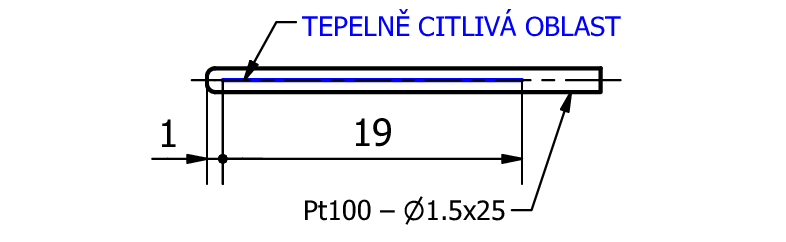
\includegraphics[width=.7\textwidth]{300_VYPOCETNI_MODEL/urceni_tr.png}
                \caption{Schéma s vyznačením oblasti odečtu teploty pro určení restitučního faktoru.}
                \label{fig:odecet-tr}
            \end{figure}

            Rovnovážná teplota $T_r$ čidla byla určena jako průměr hodnot teploty v buňkách, které úsečka protínala. Následně byl určen restituční faktor čidla s využitím Vztahu \ref{eq:mereni-rychlosti}:
            \begin{equation}
                f = 2 c_p \frac{T_r - T}{u ^2}
            \end{equation}
            \noindent kde $T \unit{K}$ je statická teplota nabíhajícího proudu a $u \unit{\frac{m}{s}}$ je jeho rychlost.

        
        